\documentclass{article}

\usepackage{fullpage}
\usepackage[utf8]{inputenc}
\usepackage{listings}
\usepackage{caption}
\usepackage{subcaption}
\usepackage[svgnames]{xcolor}
\usepackage{amssymb}
\usepackage{amsmath}
\usepackage{fancyhdr}
\usepackage{lastpage}
\usepackage{parskip}
\usepackage{abstract}
\usepackage{url}
\usepackage{float}
\usepackage{enumitem}
\usepackage{amstext}
\usepackage{fancybox}
\usepackage{amsmath}
\usepackage{graphicx}
%\usepackage{subfigure}
\usepackage[bottom]{footmisc}
\usepackage{hyperref}
\usepackage{tikz}
\usepackage{makecell}
\usepackage{tabulary}
\usepackage{pdfpages}
\usepackage{verbatim}
\usepackage{tikz}
\usetikzlibrary{positioning}
\usetikzlibrary{arrows}

\setcounter{secnumdepth}{3} % only chapter and sections will be numbered
\setcounter{tocdepth}{3}    % entries down to \subsubsections in the TOC

%%% Local Variables:
%%% mode: latex
%%% TeX-master: "report"
%%% End:

\newcommand{\code}[1]{\texttt{#1}}

%% source / reference
\newcommand{\refgeneral}[3]{#1 (#3), \emph{#2}}

% arguments:
%   author
%   title
%   year
%   publisher
\newcommand{\refbook}[4]{\refgeneral{#1}{#2}{#3}, #4}

% arguments:
%   author
%   title
%   year
%   url
\newcommand{\refonline}[4]{\refgeneral{#1}{#2}{#3} \\\url{<#4>}}

% pseudo code environment
\lstset{
  keywordstyle=\color{blue},
  commentstyle=\color{ForestGreen},
  stringstyle=\color{Maroon},%
  basicstyle=\ttfamily\small,
  frame=single,
  framesep=10pt,
  xleftmargin=30pt,
  xrightmargin=30pt,
  showspaces=false,
  showstringspaces=false,
  tabsize=4,
  aboveskip=10pt,
  belowskip=10pt,
  lineskip=2pt,
  numbers=left,
  numberstyle=\tiny,
  stepnumber=1,
  numbersep=5pt,
  breaklines,
}

\lstnewenvironment{pseudo}[1]{%
\lstset{morekeywords={if, then, else, return, function, var, for, foreach, do, end}}}%
{}

\pagestyle{fancy}
\fancyhf{}
\setlength{\parindent}{0pt}
\setlength{\headheight}{15pt}
\setlength{\headsep}{25pt}
\lhead{02122 Software Technology Project}
\rhead{The Kite Programming Language}
\cfoot{Page \thepage{} of \pageref{LastPage}}

\begin{document}

%%% Local Variables:
%%% mode: latex
%%% TeX-master: "report"
%%% End:

\newcommand*\formatname[2]{
  \leavevmode
  \rlap{\textit{#1}}
  \hspace{0.3\linewidth}
  \code{#2}}

\begin{titlepage}

\thispagestyle{empty}

\begin{flushright}
  
\includegraphics[width=9cm]{images/dtu}
\end{flushright}

\vskip20mm
\begin{center}
  
\includegraphics[width=3cm]{images/logo-clean}\\
  \vskip5mm
  \huge\textbf{The Kite Programming Language}
  \vskip5mm
  \Large 02122 Software Technology Project
  \vskip3mm
  \large June 2014
\end{center}
\vfill

\begin{flushleft}
  \normalsize
  \formatname{Simon Altschuler}{s123563} \par
  \formatname{Markus Veie Færevaag}{s123692} \par
  \formatname{Christian Mathias Rohde Kiær}{s123812} \par
  \formatname{Patrick Gadd}{s113491} \par
  \vskip2cm
  
\includegraphics[width=7cm]{images/dtu-compute}
\end{flushleft}

\end{titlepage}

\clearpage

\section*{Abstract}
\label{sec:abstract}
%%% Local Variables:
%%% mode: latex
%%% TeX-master: "../report"
%%% End:

Programming languages are the interface by which humans interact with machines. These languages come in various shapes, forms and sizes, but the one thing they have in common is that they are all implemented through some sort of compiler. This report describes how we planned, designed and implemented a compiler, and thus created the Kite programming language. With that, the general aim of the project is to gain an understanding of compilers and programming languages, with a deepened comprehension of functional programming.

We start by presenting a general overview of compilers, properties of functional programming and an outline of the steps it takes to implement one. Thereafter, we specify our requirements of the language and compiler to be implemented. These will include fundamental features of pure functional languages and systems for validating the correctness of the written code.

In the first part of the design, we start by describing the language features of the Kite programming language. Here we show that the simplicity of functional programming is a very powerful concept, that can be utilized to write expressive and concise code. To exemplify, we use runnable snippets of code, written in Kite itself, to clearly highlight the purpose and value of each feature. We move on to outlining the different components of a compiler, and what specific role each component has. This will show how every component is invaluable for building a stable compiler.

Finally, we describe in detail how we have chosen to implement the language. Here we use the Haskell programming language to step by step build a compiler from the ground up, utilizing the knowledge we have already gained through the planning process. Here it will be clear how a language like Haskell, is a good choice of language, since it already utilizes many of the features Kite will come to master. We also describe what further development on the compiler could lead to, and how we would have done it.

In conclusion, throughout the process of planning, designing and implementing the Kite programming language, we have gained a thorough understanding of compilers and functional programming languages. This is demonstrated by the functioning product that is Kite.

\clearpage

\section*{Acknowledgments}
\label{sec:acknow}
%%% Local Variables:
%%% mode: latex
%%% TeX-master: "../report"
%%% End:

TODO: Acknowledgements - det var nice at Probst gad at tage projektet!

\section*{Expected of the reader}
The reader of this report is expected to be familiar with basic functional programming and to have a notion of the most commonly used patterns such as mapping, folding and functional composition.


\section*{Breakdown of work}
TODO
\clearpage

\tableofcontents
\clearpage

\section{Introduction}
\label{sec:intro}
\subsection{Programming languages and compilers in general}

Programming languages are the means for programmers to express what the machine should compute, or in other words: What a program should do.
The two main divisions between programming languages are likely whether they are High- or Low-level and which `programming paradigm' they follow (in subsection \ref{sec:paradigms} these paradigms will be shortly described).

The low-level languages are close to what the computer `natively' understand, which is machine code/instructions, but are harder for humans to read and write. Examples hereof are FOTRAN and COBOL. Usually high-level languages are used for faster development, better readability and maintenance, among other things. Thus for many purposes programmers prefer higher level languages. These languages have to be translated into something the machine can interpret, and this is done with a so-called compiler.

A compiler is a program that translates source code in a specific language into another, usually lower level language. Thus a programming language is in fact implemented through a compiler.

\subsection{Programming paradigms}
\label{sec:paradigms}
Through the history of computer science, many different approaches to the design and implementation of programming languages have been taken. Most languages can be categorized as being either in the imperative or declarative style. Code written in imperative style is more explicit in \emph{how} a problem is solved, where declarative languages tend to describe \emph{what} is to be computed. There exists multiple language paradigms that fall under one or both of these categories.

A very popular paradigm is \textbf{object-oriented} programming (including \code{C++} and \code{Java}), in which data and algorithms are structured into objects that contain methods that can change the state of data in objects.

Another imperative approach is \textbf{procedural} languages like \code{C}, which is somewhat simpler and is characterized by subroutines, scoped variables and some sort of modules.

A very different style is the highly declarative \textbf{logic} programming, in which execution order and control-flow does not exist, but programs consist of logic clauses that define relationships and implications.

The final paradigm we will describe is \textbf{functional} programming. This is another declarative approach, which is characterized by functions and their composition as the fundamental means of expressing computations. Often programs are written in such a way that most functions are pure, meaning that they will \emph{always} return the same output given the same input.

\subsection{The problem}
The goal of this project is to gain knowledge in a field which we have only little prior knowledge about, as we at the beginning of this project have not had any formal education within the subject. In short we strive to get a good understanding of the concepts of functional programming and compilation of programming languages in general. We will achieve this by implementing a compiler for a functional language named Kite.

\subsection{The structure of the report}
The report is structured such that it somewhat follows the steps we have taken from idea to working product. We initially describe the problem and purpose of the project (chapter \ref{sec:probanal}), and then define what our requirements for completion are (chapter \ref{sec:requirements}). Next we will talk about the syntactic and semantic design of the Kite language (chapter \ref{sec:kite-design}) and how we architecturally designed the corresponding compiler (chapter \ref{sec:compiler-design}). Then follows an in-depth explanation of the implementation of each of the involved modules and their purpose (chapter \ref{sec:impl}). Finally we evaluate how the implementation turned out (chapter \ref{sec:evaluation}) and discuss what further development of Kite could lead to.

%%% Local Variables: 
%%% mode: latex
%%% TeX-master: "../report"
%%% End: 

\clearpage

\section{Problem analysis}
\label{sec:probanal}
%%% Local Variables:
%%% mode: latex
%%% TeX-master: "../report"
%%% End:

\subsection{Purpose of the project}
Our project is not concerned with solving a specific problem related to compilation of functional programming languages. Rather, it is a project in which we aim to gain a thourough understanding of modern compiler theory and implementation, as well as become proficient with functional development. We have made an effort to implement the compiler using modern techniques. That said, a compiler is a very complex piece of software and given our limited time, it is far beyond our scope to implement a language that could be used for production purposes. What we are striving to achieve, is to implement a working language with all the elements of a basic functional language, expressive syntax, simple optimizations and target language that we can execute.

There are two main aspects of the project. One is that of functional programming language theory and design, the other is that of compiler implementation and techniques. Even though they are very intertwined in the implementation, we will often touch on the two aspects separately.

Next, we will describe some properties of functional languages and compilers that we would like to implement in Kite. Further, we will introduce some of the notation used throughout the rest of the report.

\subsection{Properties of functional languages}
We will describe function types using the following notation: let $f$ be a function with a domain of $Int$ and codomain of $Float$. We denote this using '$:$', meaning ``of type'' or ``has type''.

\[ f: Int \to Float \]

Note that the concrete types are capitalized, and we use small letters to indicate type variables, also known as polymorphic types. For instance, $f: a \to b$ denotes a function which takes any type $a$ to any type $b$, and $f: a \to a$ denotes a function that takes any type $a$ and produces \emph{the same} type $a$.

The function operator $\to$ can be chained for a function to accept multiple parameters which we indicate as $f: a \to b \to c$. It's important to note that $\to$ is a \emph{binary} and \emph{right-associative} operator, meaning that

\[ f: a \to b \to c \quad \equiv \quad f: a \to (b \to c) \]

This effectively means that a function always takes exactly one argument and produces another function. In the example above, the returned value is a new function with type $b \to c$, which can then be applied to a value of type $b$ producing a final value of type $c$.

If we group the function operator differently, we can describe functions that take other functions as argument. Consider for example $f: (a \to b) \to c$, indicating that $f$ takes a function of type $a \to b$ and returns a value of type $c$. The possibility to apply functions to functions and produce functions as return values is known as \emph{higher-order} functions.

Closely related is the concept of functions as so-called \emph{first-class citizen}, which basically means that a function can be passed around and transformed just like any other type.

We consider all functions to be \emph{anonymous}, meaning that they do not have a name associated with them in their definition. They can then be bound to names using the \emph{bind} operation (syntactically denoted $=$). The following are examples of how we define concrete implementations of functions (later we will use Kite specific syntax, but for now we stick with simple mathematical notation).

\begin{align*}
id &= \fn{x}{x} & \text{The identify function: returns the argument, unchanged}\\
add &= \fn{ x, y }{ x + y }  & \text{Sum of two values}\\
max &= \fn{ x, y }{ \ite{x > y}{x}{y} }  & \text{Maximum of two values}\\
\end{align*}

Here we use the $\lambda$-notation for functions, using the ``maps to'' operator $\mapsto$ to indicate concrete implementation. We indicate function application using standard parenthesis, for instance $sum = add(2, 5)$.

A very powerful concept that arises naturally from that of higher-order functions, is that of partial application and currying. With partial application it is possible to apply a single argument to a function which takes multiple arguments, which produces a new function that accepts the remaining arguments. For instance, given the function $add$ from above, we can create a new function:
\begin{align*}
increment &: Int \to Int\\
increment &= add(1)
\end{align*}

$increment$ takes an $Int$ as argument and returns the argument, plus one. Currying is closely related, but is concerned with transforming a function of type $f : a \times b \to c$ to the function $f' : a \to b \to c$, thus enabling partial application. Here we used another notation, namely $\times$, which denotes the Cartesian product of two values, which we will further describe as a \emph{pair} of values.

As can be observed from the above, functional languages are closely related to lambda calculus, and can be seen as an extension. Common to them both is that almost everything is regarded as an expression, meaning that everything conveys a \emph{value}. For instance, in imperative languages the \code{if} construct is a statement, controlling flow of execution, whereas in a functional language, it expresses a choice between two values.

When working in an imperative language, mutation of variables is a core feature that is used in almost all parts of a program. In a functional language however, it is common that variables are not in fact variable in the sense of being mutable, but rather declarations of values. For instance, to calculate the sum of a list of numbers, consider the following pseudo-code:

\begin{pseudo}
// imperative style
function sum(nums) do
  var s = 0
  foreach num in nums do
    s = s + num
  end
  return s
end

// functional style
function sum(nums) do
  return if length of nums is 0
    then 0
    else head(nums) + sum(tail(nums))
end
\end{pseudo}

Here we can see how the imperative code continuously mutates the \code{s} variable, whereas the functional code instead leverages recursion (and also is an example of the previously mentioned \code{if} as an expression).

The idea of immutability is related to the strive for controlling side effects. In a purely functional language, a function will \emph{always} produce the same value, given the same input. This makes the code much easier to reason about, as one does not have to worry about what state a certain function is in at a given time. It can also help the compiler make optimizations, which we will discuss in more detail later. Pure languages are, however, not practical for writing useful programs because, for instance, IO is inherently not pure. You cannot know in advance what input the user will give you, and a truly pure function cannot generate random numbers, get the time, etc. Solutions have been developed to keep a language pure while still maintaining side effecting operations, such as IO. For instance, Haskell uses the concept of Monads to force side effecting functions to declare which effects they might have and provide fallback strategies in case of failure.


\subsection{Implementing a compiler}
Most modern compilers are built using more or less the same architecture. The source code of the compiled language is first analyzed lexically (a process sometimes referred to as \textbf{lexing}) into a stream of lexical tokens. This can be compared to splitting a natural language text into a list of words. This stream of tokens is then parsed into nodes in an Abstract Syntax Tree (AST), using a \textbf{parser}. This can again be compared to natural languages by imaging a list of words and punctuation being parsed into phrases that have ``meaning''.

The AST can have various forms and structures, but most commonly it is a representation of the source code in the form of data structures native to the language of implementation. The AST can be transformed for different purposes, for instance, to give correct precedence to operators.

Going further, it can be analyzed in many different ways, for example to perform \textbf{type checking} and ensure that no undefined identifiers are referenced. It is also possible to perform various optimizations on the AST. Dead (unused) code can be detected and removed, common patterns of code can be transformen into a more efficient structure, functions can be inlined to remove the overhead of making a function call and much more. This will be discussed in detail later.

Finally, the AST can be used to emit code for the target language of the compiler, a process known as \textbf{code generation}. It is worth noting that many different code generators can be implemented for the same AST, to enable targeting of multiple architectures and machines using the same compiler.

We are going to implement all of these modules, some more thoroughly than others, and in such a way that it can be easily extended and maintained.

\clearpage

\section{Requirements}
\label{sec:requirements}
%%% Local Variables:
%%% mode: latex
%%% TeX-master: "../report"
%%% End:
In the requirements-section we will focus more on the language specific features of Kite. As most of the compiler specific requirements are discussed in the design-section, and are basic for most compilers, they will not be discussed here.

\subsection{Minimum requirements}
As of our initial requirements for Kite, we have set a list of minimum requirements for our compiler.

\textbf{Type system:} Standard types that should be included in Kite is as follows:
\begin{itemize}
\item [--] Float
\item [--] Integers
\item [--] Characters
\item [--] Boolean
\item [--] Lists
\item [--] Pairs
\end{itemize}

\textbf{Static type check:}
In our initial analysis, we want to implement a static type-checker. This will ensure type safety in a given program, i.e.\ a program passing the static type-check will be free of type errors. If a program is verified by the analyzer, the compiler will be able to trust the intermediate representation given from the type-checker. This will also result in any type error will be caught compile-time.

\textbf{Code generation:}
For a machine to be able to understand the high-level language, the process of code generation is needed. Kite's code generator must be able to take some representation of the given source code, and convert it such that the machine will be able to execute the resulting output.

\textbf{Recursion:}
As recursion is one of the main properties of a functional language, it will have to be a central aspect of Kite. In general, recursion is the method of dividing a problem into sub-problems. This is top-down approach to problem-solving and is commonly referred to as the technique ``divide and conquer''. A more specific example of recursion is a function calling it-self until one or more given base-cases are met. One of the most used examples of recursion is the computation of Fibonacci numbers. As a Fibonacci number is defined as the sum of the two previous numbers, it easily implemented with recursion (albeit this particular implementation is very inefficient):

\begin{pseudo}
// fibonacci
function fibonacci(n) do
  return if n < 2
    then n
    else fibonacci(n - 1) + fibonacci(n - 2)
end
\end{pseudo}


\subsection{Optional features}

\textbf{Standard library:}
Inspired by Haskell's prelude~\footnote{\url{http://hackage.haskell.org/package/base-4.7.0.0/docs/Prelude.html}}, we want to implement a standard function library, imported by default into all Kite modules. This standard module should include useful functions for common operations as arithmetic operations, string manipulations and list manipulation.

\textbf{REPL:}
A Read-Eval-Print-Loop, or an \emph{interactive top-level}, will allow a user to have a simple interactive program to give simple input, e.g. a single expression, evaluate it and get the return value, without creating an file and compiling it.

\textbf{Higher-order functions:}
The language should provide the possibility to create function that take functions as parameters, and returns functions.

\textbf{Immutability:}
In a pure functional language there will be immutability.
TODO


\textbf{Currying:}
As we want all functions only to take one parameter, we want to include currying.
TODO: Mention lambda calculus somewhere, Hindley Milner...

\textbf{Partial application:}
As a result of currying, we want to make use of partial application. E.i. construct the foundation of function in such a way that a function takes a fixed number of arguments, returning a new function of smaller arity~\footnote{The number of arguments or operands the function or operation accepts}.

\textbf{Closures:}
The principle of closures is that when a function is referenced, it is referenced together with a \emph{referencing environment}. This environment includes a table of all non-local variables of that function. This allows a function access to non-local  variables also when invoked outside its immediate lexical scope.

\textbf{Lazy evaluation:}
The language should include lazy evaluation, which will allow evaluation of expressions to be delayed until it's needed. This technique can greatly decrease the run-time of certain code patterns.

\textbf{Type inference:}
This is an extension of the type-checker. Type inference will let the analyzer automatically deduct types of expressions, thus removed the need to declaring the types of the parameters and return types of a function.

\textbf{I/O:}
Input/Output is needed for user interaction between the user and computer. To make the language more usable, a minimum of I/O must be present. Optional features would be read/write from file etc.

\textbf{Syntactic sugar:}
To make some expressions and code pattern more readable, we want to implement a sugaring module. With this module, features as list comprehension can be added (see below).

\textbf{List comprehensions:}
List comprehensions is syntactic sugar for creating new lists from already existing lists, which is an extension of syntactic sugaring. List comprehensions will output new lists, as a result of some operation performed on each element of another list (or lists). It should also be possible to create a sub-sequence of the elements of another list, by implying that each element in the created list should satisfy a number of conditions.

\textbf{Preprocessing:}
To make it possible to include another file into a given program, we want to make use of a preprocessor. The preprocessor should be C-like where '\#include' is used to specify which external files to be included. A simple preprocessor will suffice, like the C-preprocessor.


% Mutaddfdfbghnjghfhgrbhgfdghfdvfdgbhgfdghtdehgfhgfdfbgfdbility
% REPL
% StdLib
% HoF
% Rekursion
% String interpolation
% Closures
% Lazy eval
% Parallel
% Currying
% Type system (static, strong)
% *Type inference
% I/O
% “alt = expressions”
% List comprehension
% (else?)

% TODO:
% Language features:
% Conditionals
% Functions
% “let … in”
% Loops (boobs)
% Pattern matchin

% Typez:
% String
% List
% Int
% Float/double
% Tuples/structs

\clearpage

\section{Design of the Kite language}
\label{sec:kite-design}
We have been inspired by many other languages when designing and
implementing Kite, most notably the GHC Haskell compiler\footnote{The
  Glasgow Haskell Compiler \url{http://www.haskell.org/ghc}}.

\subsection{Syntax}

TODO: Sugar, List Comprehensions, describe types, more on function declaration.

Basic declaration of the variables in Kite, types are inferred by the analyzer:
\begin{kite}
  
  one = 1
  two = 2.0
  truth = True
  list = [1, 2, 3, 4]
  str = "foo" 
  pair = (1, "one")
\end{kite}

The basic types will be Int, Float, Bool, Lists, Chars and
pairs.

Functional languages often make extensive use of lists, which is
indeed also the case for Kite. A list is an ordered array of items
that can be transformed in many different ways. We use a common
short-hand method for describing a list of things, using square
brackets $[\ ]$. For instance, a $List(Int)$ (pronounced ``List of
Ints'') is denoted $[Int]$ and a list of a type variables $a$ is
$[a]$. Lists can be nested, allowing $List(List(Int))$ denoted
$[[Int]]$.

The pair type is also abbreviated using $(,)$, for instance the type
$Pair(Int, Bool)$ is written $(Int, Bool)$

Strings is represented as syntactic sugar for lists of characters,
which will be discussed later.

Basic arithmetic operators in Kite and their us
\begin{kite}

  two = 1 + 1  ---->  2
  str = "foo" ++ "bar" ----> "foobar"
  xor = 10 ^ 8 ----> 2
  mod = 10 % 2 ---> 0
\end{kite}

\begin{table}[H]
\centering
    \begin{tabular}{|l|l|}
    \hline
    Operation    & Meaning              \\ \hline
    x + y        & Additition           \\ \hline
    x - y        & Subtraction          \\ \hline
    x * y        & Multiplication       \\ \hline
    x / y        & Division             \\ \hline
    x**y         & Exponentiation       \\ \hline
    x \% m       & Remainder of x / y   \\ \hline
    pow(x, y, m) & Modulo exponentation \\ \hline
    \end{tabular}
\end{table}

Basic boolean operators:
\begin{kite}
  
  foo = 1 < 2  ----> True
  bar = 1 == 2 ----> False
  baz = 1 != 10 ----> True
\end{kite}
Basic boolean operators include 
\begin{table}[H]
\centering
    \begin{tabular}{|l|l|}
    \hline
    Operation & Meaning                 \\ \hline
    $==$        & equal                   \\ \hline
    $/\ =$        & Not equal               \\ \hline
    $<=$        & Less than or equal than \\ \hline
    $>=$        & Greater than or equal   \\ \hline
    $<$         & Less than               \\ \hline
    $>$         & Greater than            \\ \hline
    \end{tabular}
\end{table}

basic bitwise
\begin{kite}
  
  xor = 10 ^ 8 ----> 2
\end{kite}

TODO Conditional statements 
Function declaration in Kite:
Anonymous functions:

\begin{kite}
  
|ArgName, ... | -> { ... }
\end{kite}
Since all functions in Kite is anonymous, a function is simply a
variable bound to a given anonymous function. A function is declared
as follows:
\begin{kite}
  
  function :: ArgType, ... -> ReturnType
  function = |ArgName, ... | -> { ... }
\end{kite}
Example of valid function declaration in Kite, taking one parameter of
the type Int and returning an Int.
\begin{kite}
  
  foo :: Int -> Int
  foo = |a| -> {
    a + 1
  }
\end{kite}
A runnable program must always include a main function:
\begin{kite}
  
  main = -> { ... }
\end{kite}
Using a preprocessor to include another code file, use the \#include
keyword:
\begin{kite}
  
  #include "foo.kite"
\end{kite}

By using a sugaring module, Kite will be able to express certain
functions more clearly and readable. Syntactic sugar includes infix
operators, multiple parameters on function calls, list of characters
as strings and list comprehensions.

infix:
\begin{kite}
  
  foo = 1 + 2
\end{kite}

Desugar

\begin{kite}

  foo = ((+) (1)) (2)
\end{kite}

multiple parameters:
\begin{kite}
  
  foo = |a, b| -> {
    a + b
  }
\end{kite}
desugar:

\begin{kite}

  foo = |a| -> {
    return |b| -> {
      return ((+) (a)) (b)
    }
  }
\end{kite}
Strings 
\begin{kite}
  
  str = "Hello"
\end{kite}
Desugar:
\begin{kite}
  
  str = ["H", "e", "l", "l", "o"]
\end{kite}

\label{sec:ex-listcomp}
List comprehensions are syntactic sugar for manipulating
lists. An example of a list comprehension is as follows:
\begin{kite}
  
  list = [ x*y | x <- range(3,5), y <- range(4,6) | (x+y) >= 10, y > 4]
\end{kite}
where the desugared version of the same example, will look as follows:
\begin{kite}

  list =
  flatMap(|x| -> {
    flatMap (|y| -> {
      if (|x,y| -> {y > 4})(x,y) && (|x,y| -> {(x+y) >= 10})(x,y) 
         then [(|x,y| -> {x*y})(x,y)] 
         else []
    } , range(4,6) )
}, range(3,5) )
\end{kite}
Take note that list comprehensions uses functions defined in the
foundation, which will be discussed later
\subsection{Semantics}

TODO: Recursion, HoF, Currying, pattern matching,
partial application, Mutability. maaske mere.

Example of pattern matching
\begin{kite}

fibo = |a, b, n| -> {
    match n {
    0 -> a,
    n -> fibo(b, (a + b), (n - 1))
    }
}
\end{kite}

\subsection{Foundation}

As earlier mentioned, the foundation of Kite is a standard library
consisting of often used functions. Kites foundation is inspired by
Haskells prelude, and includes many functions found in prelude.
TODO: MORE FUN FUN FUN

%%% Local Variables: 
%%% mode: latex
%%% TeX-master: "../report"
%%% End: 

\clearpage

\section{Design of the compiler}
\label{sec:compiler-design}
To describe the overall design of the Kite compiler, we will start by
breaking it down into general parts, where each part or module has a
specific task. Below we have a waterfall model including the main
parts of the compiler:

\begin{figure}[H]
  \label{fig:flow}
  \center
  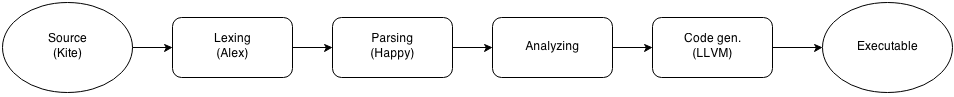
\includegraphics[scale=0.45]{images/flow.png}
  \caption{General flow of the Kite compiler}
\end{figure}

At first it can seem a little daunting, but when we get into the
purpose of each step, there will be a more obvious flow.

\subsection{Preprocessor}
The first thing the compiler does is preprocess the input, e.i. the
source code files, that it has been given. This is quite simply the
task of including all necessary files into one file. The files to be
included are declared in the top of the file.

\begin{figure}[H]
  \label{fig:preprocessor}
  \center
  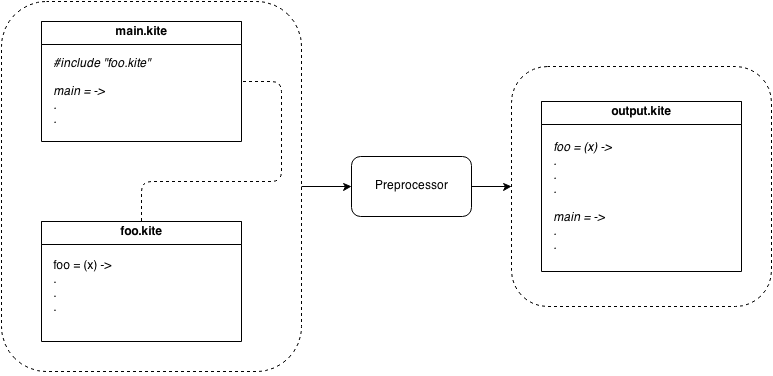
\includegraphics[scale=0.45]{images/preprocessor.png}
  \caption{Input and output of the Preprocessor}
\end{figure}

The nature of the preprocessor is quite simple, as the only task it
simple textual substitution.

\subsection{Lexical analysis}
The lexical analyzer, or just \emph{lexer}, is a central part of most
compilers. It has the important task of processing some input and
converting it to known, referencable tokens. This process is commonly
known as \emph{tokenization}.

Most lexers are quite simple, as they simply make tokens by matching the input with regular languages and classify the substrings according to these. Thus lexers do not perform any complex tasks - this is reserved for the parser and analyzer, which we will describe in the following.


\subsection{Parser}
The parser takes the list of tokens from the lexer and based on a
language grammar, it builds a corresponding data structure, namely the
parse tree. In the process it checks that that the input is
syntactically correct. Therefore, this process is also called syntactic
analysis.

In the cases know to us (Yacc, Happy, ANTLR), parser-generators make use of \emph{Context-Free Grammars} (CFG), and thus we have to define our desired syntax as a CFG.

The parser should rule out code containing syntactical errors, especially typos, which are likely to occur without a good IDE\footnote{IDE is short for Integrated Development Environment, which, among other features, often has good auto-completion, thus making typos much less likely.}.

\subsection{Desugar}
In order to make the language more convenient to write, we have made syntactic sugar and will introduce a desugaring module. This will take specific syntactic constructs and convert them into their more basic elements.

\subsection{Analyzer}
The analyzer will traverse the parse tree and perform \emph{typechecking} and look for calls to undefined functions. The analyser should spot almost all remaining incorrect code. Thus the output should be able to be executed without errors due to incorrect types, typos or the usage of undeclared variables.

The analyzer cannot, however, determine whether a program will yield the expected results or even if it will ever terminate.


\subsection{Optimizer}
The optimizer module takes the AST and can perform optimizations on it. This is described in more detail in section \ref{sec:impl-optimizer}.


\subsection{Code generation}
The code generator will take the AST outputted from the parser, and emit code for a specified target language. Currently Kite only supports one code generation backend namely for JavaScript, but the module is structured in such a way that allows easy integration with new code generation modules.

\textbf{LLVM as backend:} The LLVM compiler
infrastructure\footnote{LLVM Project \url{http://llvm.org/}} will allow
for low level binary machine code generation. The LLVM infrastructure
will take a representation of the parse tree and emit a LLVM
intermediate representation (IR) which can be used for code
generation. Since LLVM is strong statically typed, a modified variant
of Kites parse tree is needed. The LLVM infrastructure will also provide
optimization passes for a given LLVM IR.

\textbf{JavaScript as backend:} As an alternative, a JavaScript emitter
can be implemented and used as backend. Since JavaScript is untyped,
Kite can rely on the typechecker and emit JavaScript. The emitted
JavaScript should not contain type errors, as the analyzer will
catch type errors. The emitted JavaScript will run on the
Node.js platform\footnote{ The Node.js platform \url{nodejs.org}}.
Node.js makes use of the Google V8 JavaScript engine \footnote{Google
  V8 engine \url{http://code.google.com/p/v8/}} which compiles JavaScript to
native machine code. The result is faster and more optimized
JavaScript execution.

%%% Local Variables:
%%% mode: latex
%%% TeX-master: "../report"
%%% End:

\clearpage

\section{Implementation}
\label{sec:impl}
%%% Local Variables:
%%% mode: latex
%%% TeX-master: "../report"
%%% End:

\subsection{Preprocessor}
The preprocessor in Kite is almost identical to the \code{C} language preprocessor. We use a library called \code{cpphs}~\cite{wallace04}, which is a port of the \code{C} version, and provides an embeddable Haskell library. This is the reason for the \code{\#include "file.kite"} syntax. Preprocessing is the initial step of the compilation, and generates a single source code file which is a recursive concatenation of all included source files referenced from the main file.


\subsection{Lexer}
\label{sec:impl-lexer}
The lexer converts the raw input source to a list of tokens, a process known as tokenization. There are multiple types of tokens that represent different kinds of lexical elements. A \emph{lexeme} is the textual value that the lexer sees and maps to a token. Some tokens can have multiple possible lexemes, for instance in the case of identifiers and numeric constants. In those cases, the lexeme is saved together with the token for further evaluation (by the parser).

Kite's lexer is implemented using the lexical generator, Alex~\cite{dornan01}. Alex is a tool for generating lexical analyzers in Haskell, given a description of the tokens to be recognized in the form of regular expressions~\cite[p. 4]{dornan01}. The description of the analyzer consists of \emph{macro definitions} and \emph{rules}. A macro definition is either a regular expression bound to an identifier describing a particular sequence of characters, denoted by a \code{\$} prefix, or it is a combination of the former, prefixed by \code{@}. These macros are combined to make up the rules, which define the actual definitions for tokens. Macros and rules are separated by the symbol \code{:-} and the preceding \code{kite} is just for documentation~\cite[p. 7]{dornan01}. Further the description file defines the Haskell data structures used to represent the tokens, enclosed in '\code{\{ \}}'.

Figure~\ref{fig:lexer} shows an excerpt from the description file (\code{Lexer.x}). The macro definitions describes common patterns such as a sequence of digits (\code{\$digit}), lowercase characters (\code{\$downcase}), alpha numeric sequences (\code{\$alphaNum}) etc. Also defined are reserved keywords (\code{\@keywords}) and the void type (\code{@void}). Another interesting macro is the \code{@comment} macro, which matches two dashes followed by anything (implicitly anything but a newline).

The macros are then used in the rules to define tokens. A rule consist of a combination of macros followed by a Haskell code block that produce the token data structure. The code block must be a function accepting a position data structure and the matched lexeme. The position node is used to keep track of tokens where found in the source file to be able to give useful error messages. The lexeme is sometimes coerced to another value matching the one required by the respective token structure. The \code{@void} rule defines the \code{Void} type which is the only token possible from that rule, and therefore it ignores the provided lexeme.

Note that the (\code{@comment}) rule defines no code block but just a \code{;} which means that the pattern is matched, consumed and ignored, which is exactly what we want for comments.

At the bottom we see the data constructors used to create the tokens.

\begin{figure}[p]
\begin{lstlisting}
$downcase		= a-z
$upcase			= A-Z
$digit			= 0-9
$alpha			= [$downcase $upcase]
$alphaNum		= [$alpha $digit]

@keywords		= return | if | then | else | match
@identifier		= $downcase [$alphaNum \_ \' \! \?]*
@void           = Void
@comment		= "--" .*

kite :-
  @comment		    ;
  @keywords		    { \p s -> TKeyword p s }
  $digit+\.$digit+	{ \p s -> TFloat p (read s) }
  $digit+		    { \p s -> TInteger p (read s) }
  @identifier		{ \p s -> TIdentifier p s }
  @void		        { \p s -> TVoid p }

{
data Token = TIdentifier AlexPosn String
           | TInteger    AlexPosn Int
           | TFloat      AlexPosn Float
           | TKeyword    AlexPosn String
           | TVoid       AlexPosn
           deriving (Eq,Show)
}
\end{lstlisting}
\caption{Excerpt from the lexer description file}
\label{fig:lexer}
\end{figure}

Kite uses 12 different tokens briefly described in table~\ref{tbl:lexical_tokens}.
\begin{table}[H]
  \centering
  \begin{tabular}{lll}
    \textbf{Token} & \textbf{Description} & \textbf{Sample lexemes}    \\ \hline
    Symbol     & Single character symbols & \code{;, !} \\ \hline
    Identifier & Identifiers for referencable variables & \code{map, x', \_foobar} \\ \hline
    Type       & Capitalized identifier, denoting a type construct & \code{Bool, Int, Void} \\ \hline
    Integer    & Integer sequence & \code{0, 1, 1337}\\ \hline
    Float      & Floating point values & \code{0.0, 3.14, 2f} \\ \hline
    Bool       & Boolean values & \code{True, False} \\ \hline
    Void       & The void type & \code{Void} \\ \hline
    String     & Sequence of characters enclosed in \code{``''} & \code{``Hello, world!''} \\ \hline
    Char       & Single character enclosed in \code{\'} & \code{'a', '!', ' '} \\ \hline
    Keyword    & Reserved keywords used in the Kite syntax & \code{if, return, match} \\ \hline
    Operator   & List of symbol characters & \code{=, /, <=, !!} \\ \hline
    EOF        & The end of file marker & n/a as it's non-visual
  \end{tabular}
  \caption{Tokens recognized by the lexical analyzer}
\label{tbl:lexical_tokens}
\end{table}


\subsection{Parser}
The parser is implemented with the LALR-parser (\textbf{L}ook \textbf{A}head, \textbf{L}eft-to-Right, \textbf{R}ightmost derivation) generator Happy~\cite{marlow01}, which is a parser generator system for Haskell, similar to the tool Yacc\footnote{Yacc: Yet Another Compiler-Compiler: \url{http://dinosaur.compilertools.net/yacc}} for C. It takes a file containing a specification of a grammar and produces a Haskell module containing a parser for the grammar. The grammar file (\code{Parser.y}), is similar in format to the lexical analysis description file described in section~\ref{sec:impl-lexer}. It uses Backus-Naur Form (BNF) notation to define a context-free grammar specifying the legal syntax of the Kite language. A BNF grammar consists of a set of derivation rules, also known as production rules, which describe all legal combinations of the tokens read by the lexer. A production rule has the following format:

\begin{lstlisting}
Name :: { Type }
      : Expression_1 { Haskell code }
      ...
      | Expression_n { Haskell code }
\end{lstlisting}

The \code{Type} specifies the type of Haskell data constructor that the rule will produce and is optional, but useful for debugging purposes and readability. A rule can have multiple different legal expressions, separated by \code{|}, which are defined as a sequence of symbols. A symbol can be either a \emph{terminal} or another production rule. A terminal is an expression that cannot be further expanded, thus terminating the recursion of that branch. For instance, consider the production rule for the bind syntax (the bind node is named \code{PBind} in the Haskell code).

\begin{lstlisting}
Bind :: { Expr }
      : id '=' Expr                  { PBind $1 $3 }
      | '{' operator '}' '=' Expr    { PBind $2 $5 }
\end{lstlisting}

The \code{Bind} rule produces a node of type \code{Expr}. In the first choice we see the \code{id} terminal that is equivalent to the \code{Identifier} token from the lexer. Other terminals are \code{'='}, \code{'\{'} and \code{'\}'}. The right-hand side of the rules are the code snippets that defines what Happy will generate when a rule is matched, where \code{\$n} means that the $n$th symbol of the BNF notated grammar, will be inserted. In the first rule this means that a \code{PBind} will be created with the \code{id} as the first argument and the \code{Expr} rule as the second.

Production rules can be recursively defined, so that an expression can contain the rule itself. Consider, for instance, the grammar for defining lists:

\begin{lstlisting}
Exprs :: { [Expr] }
       : {- nothing -}    { [] }
       | Expr             { [$1] }
       | Expr ',' Exprs   { $1 : $3 }

List  :: { Expr }
       : '[' Exprs ']'    { PList $2 }
\end{lstlisting}

The \code{Exprs} rule defines a comma-separated list of \code{Expr} rules. The \code{\{- nothing -\}} defined the empty match, equivalent to the common mathematical notation, $\epsilon$.

The first rule in the grammar defines the entry point of the parser and thus the resulting type that the generated parser will produce. In the case of Kite, the entry rule is \code{Program} that produces the type \code{[Decl]}.

\paragraph{Syntactic sugar}
Some matches are first transformed into temporary syntactic sugar structures, before being inserted into the parse tree. This is described further in section~\ref{sec:imp-sugar}.

Happy generates more than 2,000 lines of quite unreadable Haskell code, which is used in the compilation of the compiler. This is not useful for debugging, but fortunately Happy can produce an information file by setting the \code{--info} flag when run, which will generate a \code{.info}-file. This file contains very useful information about shift-reduce and reduce-reduce conflicts, which has been quite helpful throughout the development.

\paragraph{Shift-reduce parsing}
Happy generates a shift-reduce parser. This means that, when it reads a symbol, it will either reduce the symbol, thus ``ending'' a rule and producing a result, or it can shift the symbol and look for more symbols to match before reducing. This is the point of a Look-Ahead parser, since it can look at the next symbol to be consumed before deciding what to do. Happy generates LALR(1), which means that it looks 1 symbol ahead.

A common hurdle when implementing shift-reduce context-free grammars (and indeed parsers in general), is conflicts or ambiguities in the grammar. There are two types of conflict, namely \emph{shift/reduce} and \emph{reduce/reduce} conflicts. A reduce/reduce conflict occurs if there are two or more rules that apply to the same sequence of symbols~\cite[sec. 5.6]{bison13}.

When the parser sees a symbol and can \emph{reduce} to two different rules, it is called a reduce-reduce conflict. This is usually a critical problem because the parser has no reasonable way of choosing which rule to reduce to. Happy simply reduces to the rule defined first. Below is the simplest example of a reduce/reduce conflict (in simplified BNF notation).

\begin{lstlisting}
Foo : 'a'
Bar : 'a'
\end{lstlisting}

When seeing an \code{'a'} the parser cannot decide whether to reduce to \code{Foo} or \code{Bar}.

A shift-reduce conflict happens when the parser has the option to either reduce a rule or shift the symbol and continue. This is much less critical because the desired choice is almost always to shift. Consider the following example of $a$.

\begin{lstlisting}
Foo : 'a' 'b'
Bar : 'a'
\end{lstlisting}

Here the parser, when seeing an \code{'a'} as the current symbol and \code{'b'} as the look-ahead symbol, can either reduce the \code{Bar} rule or shift the \code{'a'} and continue parsing the \code{'b'}.


\subsection{Syntactic sugar}
\label{sec:imp-sugar}
Because of the simplistic nature of the Kite AST, it would be terse to write programs that directly translate to AST nodes. The \code{Desugar} module allows Kite programs to be written in a succinct manner and further enables a powerful feature known as \emph{list comprehension}. It makes the language ``sweeter'' for human use; things can be expressed more clearly, more concisely, or in an alternative style that some may prefer~\cite{wiki-sugar14}. The process of converting sugared syntax to standard form is called \emph{desugaring} of code.

We have decided to integrate desugaring directly in the parser because this avoids the need for an intermediate AST representation to be desugared after parsing. The \code{Desugar} module defines functions to desugar specific cases of sugar, that are used in the Haskell code snippets. For instance in the rule for function application, \code{Apply}:

\begin{lstlisting}
Apply :: { Expr }
      : Expr '(' Exprs ')'    { mkCalls $1 $3 }
      | Expr '`' Expr Expr    { PApply (PApply $3 $1) $4 }
      | ...
\end{lstlisting}

Here the function \code{mkCalls}, defined in the \code{Desugar} module, converts multiple arguments to a function, to a series of applications. Most of the desugaring is straight forward and the details of their use is described in section~\ref{sec:kite-design-sugar}, but we will explain the most interesting parts.

\paragraph{Strings}
As the representation of strings outputted from the lexer is a Haskell \code{String} type (which is a type synonym for \code{[Char]}), we simply map the \code{PChar} constructor over each letter and construct a \code{PList} containing the resulting list. This way, a string ends with having the type \code{PList PChar} in the AST.

\paragraph{Multiple arguments in function application}
The \code{mkCalls} function converts a function call with multiple arguments to a sequence of applications.

\begin{haskell}
mkCalls f [] = PApply f PVoid
mkCalls f (a:as) = foldl PApply (PApply f a) as
\end{haskell}

Where \code{(a:as)} is the destructured list of arguments, we reduce the list by folding with a \code{PApply} data constructor.

\paragraph{List comprehensions}
As list comprehensions are composed of an output expression, draws and guards, the desugaring is implemented as follows (for an example of a list comprehension, and its desugared version, see section~\ref{sec:ex-listcomp}):

\begin{enumerate}
\item The identifiers from the draws are extracted as these will be used as arguments to the various functions.

\item A \code{flatMap}\footnote{\code{flatMap} takes as arguments a lambda-expression and a list, maps the function over the list, and \code{flatten}s the result} function is generated for each of the draws, taking the identifier of the current draw and the list-expression as defined on the right-hand side of the \code{<-} (e.g. \code{[1, 2, 3]} in \code{x <- [1, 2, 3]}) as arguments. The body of the lambda expression is either a nested \code{flatMap} or the final if-expression as generated from the guards:

\item The guards are inserted as individual functions which take all the extracted identifiers as arguments. These lambda-expressions are then conjoined in the condition of the \code{if}-expression.

\item The \code{then}-branch of the \code{if}-expression is a function with the output expression as its body and the extracted identifiers as its arguments. The \code{else}-branch is simply an empty list. This implies that only the elements that pass the guards are outputted, as \code{flatMap} excludes the empty elements.
\end{enumerate}


\subsection{Analyzer}
After the front-end of the compiler has finished parsing the program, the analyzer will traverse the AST, gathering information and verifying its validity in various ways. Below we will describe the different types of analysis that our compiler implements.

\subsubsection{Type checking}
Kite uses static type checking to verify that types align at compile-time. There are numerous techniques for validating that types align and the program will not crash due to type errors. If a language forces annotations of all identifers, such as function parameters and bound variables, it is almost trivial to verify if types align since all information needed is provided by the programmer and the compiler will only have to match annotated types with literal values. Languages like \code{ML} and \code{Haskell} does not require any types to be speficied by the programmer, but it will still be able to statically check that types match. It does this by \emph{inferring} types of expressions, that is, the type of an expression can be determined simply by examining it recursively. Consider the identity function

\begin{kite}
id = |x| -> { x }
\end{kite}

What is the type of \code{id}? We cannot assign any concrete types like \code{Int} and \code{Bool} because the function does provide us with any type information at all. All we know is that \code{x} will have a type, let's call it $\alpha$, and that \code{x} is exactly what is returned, so the return type of \code{id} \emph{must} be $\alpha$ as well. The answer is thus that \code{id} has the type $\alpha \to \alpha$, where $\alpha$ is \emph{type variable}, meaning it can be substituted for \emph{any} other type, regardless whether it is another type variable or a concrete type.

This is fundamentally what \emph{type inference} does, though it becomes more difficult to grasp when formalised and performed on complex types. In the following we will explain how type checking works in Kite.

First we present some notation. We will use greek letters to indicate type variables, and latin letters to indicate identifiers. We define $:$ to mean ``has type'', such that for the above example we would write $id: \alpha \to \alpha$. When deriving types for subexpression we use $\vdash$ to mean ``implies that''. For instance $x = 1 \vdash x : Int$ is read as ``given the expression $x = 1$ we can derive that $x$ has type $Int$''. The $\to$ defines domain and codomain of a function and is a right-associative operator. Recall that all functions in Kite (and in the following) take one single argument and returns one single value. For an implementation we use the $\mapsto$ operator, and to define a lambda expression we use $\lambda$. We use the shorthand notation for the list type, namely $[\alpha]$ meaning ``list of $\alpha$''. The pair type is notated $(\alpha, \beta)$ meaning a pair containing to values of type $\alpha$ and $\beta$.

We have implemented type inference with the Damas-Hindley-Milner algorithm. They presented an algorithm, named ``Algorithm W''\cite[sec. 6]{milner82} that, given an expression will infer the \emph{principal} of that expression. A principal type is the most general type possible of an expression. Consider again the \code{id} function; $id:Int \to Int$ is valid but is not as general as $id: \alpha \to \alpha$ because it will not allow application to e.g. \code{Bool} and \code{Char} values.

To give a sense of what the algorithm will infer we present a few examples. Let the following be predefined
\begin{align*}
  add    & : \alpha \to \alpha \to \alpha\\
  head   & : [\alpha] \to \alpha   \\
  fst    & : (\alpha, \beta) \to \alpha
\end{align*}

The algorithm can now infer the types of the following expressions
\begin{align*}
  \fn{xs}{head(xs) + 1} & \qcol [Int] \to Int         & \qvd xs : [Int]                  \\
  \fn{p}{fst(p) + 1}    & \qcol (Int, \alpha) \to Int & \qvd p : (Int, \alpha)           \\
  f(add(n, 1))          & \qcol \alpha                & \qvd f: (Int \to \alpha), n: Int \\
\end{align*}

Using the last example above, the intuition behind the algorithm is as follows
\begin{enumerate}
\item $e = \fn{f, n}{\ldots} \vdash e: (\alpha \to \beta \to \gamma)$ \\
  $e$ is being assigned a lambda expression with two parameters but we do not know anything about their types, so we assign them unique type variables.
\item $e = \fn{f, n}{f(\ldots)} \vdash f: \delta \to \gamma$ \\
  $f$ is being applied to a single (yet unknown) value, thus we can infer that it is a function
\item $e = \fn{f, n}{f(add(n, 1))} \vdash n : Int$ \\
  We see that $f$ is applied to $add(n, 1)$ and since $1: Int$ and $add:\alpha \to \alpha \to a$ then $\alpha = Int$ and thus $n:Int$ (this is called type unification, explained below).
\item $e = \fn{f, n}{f(add(n, 1))} \vdash e : (Int \to \gamma) \to Int \to \gamma$ \\
  There are no more expressions to infer so we end up with the final, principal type for $e$
\end{enumerate}

\paragraph{Substitutions}
A \emph{substituion} is a set $\sigma$ of mappings from type variables to terms. A term is either a composite type, a type variable or a concrete type. The notation $\{ x_1 \mapsto \tau_1, \ldots, x_n \mapsto \tau_n \}$ denotes a substitution mapping $x_n$ to $\tau_n$. A substitution can be \emph{applied} to a term thus replacing all occurrences of variables with the corresponding type in the substitution. A term is called an \emph{instance} of a substitution after it has been applied\cite[sec. 1]{wiki-unif14}. Application is written postfix, so for instance $(\alpha \to \beta) \{\alpha \mapsto Int\} = Int \to \beta$.

Two substitutions $\sigma$ and $\sigma'$ can be composed to make a unified substitution $\sigma''$ such that $\forall x \in (\sigma \cup \sigma') | x \in \sigma''$, or in other words $\sigma'' = \sigma \cup \sigma'$

\paragraph{Type unification}
Given two type terms $t$ and $u$, the unification algorithm will either produce a substitution that \emph{unifies} the two types, i.e. some $\sigma$ such that $t\sigma = u$ or it will fail, indicating that no such substitution exists. If unification returns a substitution it will be the \emph{most general unifier} meaning the substitution that will provide the most general type when applied to the terms.

In practice the unification algorithm recursively unifies composite types. The actual Haskell implementation is very close to the following:

\begin{align*}
unify(t, u) = \begin{cases}
  \{\}                                    & \mbox{if } t == u                                    \\
  \{ t \mapsto u \}                       & \mbox{if } t \mbox{ is variable}                     \\
  \{ u \mapsto t \}                       & \mbox{if } u \mbox{ is variable}                     \\
  unify(t', u')                           & \mbox{if } t = [t'] \mbox{ and } u = [u']            \\
  unify(ta, ua) \cup unify(tb, ub)        & \mbox{if } t = (ta, tb) \mbox{ and } u = (ua, ub)    \\
  unify(tp, up) \cup unify(tr, ur)        & \mbox{if } t = tp \to tr \mbox{ and } u = up \to ur \\
  \text{failure: types are not unifiable} & \mbox{otherwise}
\end{cases}
\end{align*}

This definition of $unify$ will find the most general unifier for any two terms or fail. Note that a type variable can map to another type variable. Following are a few examples of the output of $unify$

\begin{align*}
unify(\alpha, \beta)                          & = \{ \alpha \mapsto \beta \}                             \\
unify([\alpha], [Int])                        & = \{ \alpha \mapsto Int \}                               \\
unify(Int, Int)                               & = \{  \}                                                 \\
unify(Int \to \alpha, \beta \to Int \to Bool) & = \{ \beta \mapsto Int, \alpha \mapsto (Int \to Bool) \} \\
                                                                                                         \\
unify(Int, Bool)                              & = \text{failure}                                         \\
unify(Int, [Int])                             & = \text{failure}                                         \\
unify(\alpha \to Int, Bool \to Char)          & = \text{failure}                                         \\
\end{align*}

\paragraph{Putting it together}
We have now presented a type unification algorithm and defined substitutions. We still need a system that combines these concepts and brings us a complete type-checking system.

The type-checking module \code{Kite.TypeCheck} implements an \code{infer} function that takes an expression and either returns its principal type or throws an error. The \code{infer} function evaluates in the \code{TC} monad\footnote{Monads are a functional way of, among other things, simulating state and managing errors and side effecting computations while remaining pure. We will omit details about this concept in the report.} that provides an environment for persisting inferred types and keeping track of other stateful properties such as the number of type variables created.

The type-checker is passed a list of top-level declarations and type annotations. It infers each declaration's type and validates whether it unifies with the annotated type, if one has been provided. If it successfully finds a principle type it is saved in the top of the \emph{symbol stack}. The symbol stack is a stack of maps that provide mappings from identifiers to types. When inferring the type of a lambda expression, a new \emph{stack frame} is pushed to the stack, thus beginning a new lexical scope. When all expressions in the lambda block have been processed the frame is popped from the stack, thus leaving the scope as it was.

Each time a new identifier is introduced the algorithm generates a \emph{fresh} type variable for it, meaning a type variable with an identifier that has not been used before. It does this by continuously keeping track of how many type variables have been introduces and postfixing the identifier with this value.

\code{infer} recursively traverses the AST node for which it is inferring a type while passing around a map of inferred locally scoped type variables. There is a case for each type of AST node, but we will not cover each of them in-depth, but explain the case for \code{Apply}.
\begin{figure}
\begin{lstlisting}[mathescape=true]
infer env (Apply expr arg) = do
  $\sigma_{fn}$, $\tau_{fn}$ = infer env expr
  $\sigma_{arg}$, $\tau_{arg}$ = infer env arg

  $\tau_{fresh}$ = freshTypeVar()

  $\sigma$ = unify ($\tau_{fn}\sigma_{arg}$) (LambdaType $\tau_{arg}$ $\tau_{fresh}$)

  return ($\sigma \cup \sigma_{arg} \cup \sigma_{fn}$, $\tau_{fresh}\sigma$)
\end{lstlisting}
\caption{Pseudo code of the \code{infer} function applied to an \code{Apply} node}
\label{fig:infer-apply}
\end{figure}

Figure \ref{fig:infer-apply} shows how the algorithm first infers the type of the function to be applied (line 2) and the argument it will be applied to (line 3). It then generates a fresh type variable (line 5), and unifies the inferred type of the function with a newly constructed lambda expression that has the fresh type as return type (line 7). Unless the recursive calls to \code{infer} or unification fails, it returns (line 9) the composed substitutions and the type of the lambda which is an instance of the substitutions from the unification.

This is fundamentally how the type-checker works, but there are a few noteworthy things to add. When we are retrieving a previously inferred type of a lambda expression we will \emph{freshen} its type, meaning that we replace all type variables in its type with fresh ones. If we omit this, two applications of the same function can result in the same type variable being inferred thus restricting the two inferred types to being the same type.

Finally we use implicit recursive definitions when binding an identifier to a lambda expressions. This allows recursively defined functions but prevents bindings like \code{foo = 1 + foo}.

\paragraph{Limitations of Hindley-Milner}
While the Hindley-Milner algorithm certainly is powerful and elegant, it has (in its original form) some limitations that constrain the type system. Most notably we cannot support subtyping, meaning that we cannot define a type as being an extension of another. Subtyping in \code{Java} is declared using the \code{extends} keyword, thus making a \code{class} a subtype of another class (called the supertype).

Subtyping is not possible (or difficult at the least), due to the fact that the unification algorithm cannot compute the principal type of an expression if subtypes are allowed.

\subsection{Optimizer}
\label{sec:impl-optimizer}
The optimizer of the Kite compiler is currently only a simple dead-code elimination algorithm. The algorithm is given a starting declaration (usually the \code{main} declaration) and recursively traverses the AST, beginning with the expressions defined in the starting node. When an identifier node is detected (except in a bind node) its name is saved and the recursion continues. The part of the AST which has been traversed, is the derivation tree that will be executed when running the program, thus containing all referenced identifiers. The full list of declarations is now filtered by only persisting the ones that were detected during traversal, since we can be certain that they are the only ones that can ever be referenced.

In its current state, the algorithm only eliminates unused top-level declarations, thus leaving unused locally scoped variables in the code. The algorithm can however be extended to eliminate local variables by transforming the AST during traversal. With a stack of used identifiers, we could, when entering a new local scope (a lambda or match case), push a new frame to the stack, add accessed variables found in the current scope, and when leaving the scope, filter out the variables that were not referenced.

\subsubsection{Target specific optimization}
Optimizations can be done either on the intermediate AST as above, or while emitting target code. Kite does some simple optimizations for the JavaScript target by expanding calls to common binary arithmetic operations (such as \code{+} and \code{*}). Consider the expression \code{a = 1 + 1}. Without optimization the emitted code looks like \code{var a = KT\_PLUS(1)(1)} which  requires two function calls to be evaluated. The optimized version is simply \code{var a = 1 + 1}.

In cases such as the above, we could in fact optimize further by directly calculating the resulting value as it's a constant expression.


\subsection{Code generation}
The implementation of code generation focuses on the target language JavaScript, as the initial aim of LLVM was not met. This will be discussed more thoroughly in section~\ref{sec:discussion}.

The code generation module will run recursively through the AST and emit JavaScript code for each node. This is done with the \code{emit} function, which has the type signature of \code{Expr -> Source}.

In the following we will look at some examples of different types of expressions:

Given a \code{PLambda} node, which is a function declaration, there will be generated a corresponding function decleration in JavaScript.

\begin{haskell}
emit (PLambda param body) = printf "(function(%s) {%s})" param (emit body)
\end{haskell}

Where the emitter takes a \code{PLambda} node with its given parameters and body. There will therefore be emitted a JavaScript function with the given parameters and body, where the body, of type \code{PBlock}, is recursively emitted. The \code{PBlock} node, which is usually the body of a \code{PLambda}, is emitted as follows:

\begin{haskell}
emit (PBlock exprs) = emitAll ";" exprs
\end{haskell}

The \code{PBlock} is a list of expressions, which is emitted recursively and is separated by semi-colons (\code{;}).

The \code{PBind} node, which binds an identifier to a given expression, is emitted as follows:
\begin{haskell}
emit (PBind ide expr) =
  printf "var %s = %s;" (safeId ide) (emit expr)
\end{haskell}
Here the identifier is declared as a JavaScript variable with the keyword \code{var} and it has the expression assigned to it.

If we, for instance, have the following (quite inaccurate) function:
\begin{kite}
isPrime = |n| -> {
  primes = [2, 3, 5, 7]
  n `elem primes
}
\end{kite}

The code generator will emit the following, where \code{elem} (from Foundation) is first partially applied to \code{n}, which then returns a function that is instantly applied to \code{primes}:
\begin{lstlisting}[language=Javascript]
var isPrime = (function(n) {
  var primes = [2,3,5,7];
  return elem(n)(primes)
})
\end{lstlisting}

The code generator will always embed \code{kt\_runtime.js} (see~\ref{kt-runtime}), which is Kite's JavaScript runtime environment. The runtime includes various native JavaScript functions, which can be used in Kite source code. As an example, basic I/O is included in \code{kt\_runtime.js}. This includes \code{print} and access to command-line arguments:
\begin{lstlisting}[language=Javascript]
var print = function (str) {
  console.log(_print(str));
};

var KT_arguments = function () {
 return process.argv;
};
\end{lstlisting}

\clearpage

\section{Evalution of implementation}
\label{sec:evaluation}
%%% Local Variables:
%%% mode: latex
%%% TeX-master: "../report"
%%% End:

\subsection{Development}
\subsubsection{Source code management}
Through out this project we have used git~\footnote{\url{http://git-scm.com/}} to manage the source code of the Kite-compiler and its dependencies. The repository is hosted at GitHub~\footnote{\url{https://github.com/}} and can be found publicly at \url{https://github.com/altschuler/kite}.

\subsubsection{IDE}
For development of kite code, we have made a kite-mode to integrate in Emacs~\footnote{\url{http://www.gnu.org/software/emacs/}}. This provides syntax-highlighting and various shortcuts for compilation and execution of JavaScript with Node.js.

The source of kite-mode is located in the \code{utils} directory of the repository. See~\ref{kite-mode}, for the source.


\subsection{Preprocessor}
As we use \code{cpphs}\cite{wallace04} for preprocessing, which is a port of the C-preprocessor in Haskell, one will have to take certain considerations when including files.

One major pitfall is creating circular dependencies. If two files includes each other, using the \code{\#include file.kite} syntax, this will cause an infinite loop of the files including each-other, resulting in a stack-overflow. Circular dependencies are not detected which can cause confusing errors, without any detailed feedback.

Another hurdle is including the same file twice. Take for example the following set of files and inclusions:

\begin{kite}[caption=\code{grandfather.kite}]
  foo = -> { bar }
\end{kite}

\begin{lstlisting}[caption=\code{father.kite}]
  #include 'grandfather.kite'
  ...
\end{lstlisting}

\begin{lstlisting}[caption=\code{child.kite}]
  #include 'grandfather.kite'
  #include 'father.kite'
  ...
\end{lstlisting}

This will cause a compile-time error, as the \code{foo} function is declared twice, which is not allowed.

Both of these pitfalls can be avoided using include guards~\footnote{\url{http://en.wikipedia.org/wiki/Include_guard}}, ensuring that a file is only included if a specific flag is not defined, meaning the file has not yet been included.

\begin{lstlisting}[caption=\code{grandfather.kite}]
  #ifndef GRANDFATHER_H
  #define GRANDFATHER_H

  foo = -> { bar }

  #endif
\end{lstlisting}

\begin{lstlisting}[caption=\code{father.kite}]
  #include 'grandfather.kite'
  ...
\end{lstlisting}

\begin{lstlisting}[caption=\code{child.kite}]
  #include 'grandfather.kite'
  #include 'father.kite'
  ...
\end{lstlisting}


\subsection{Tests}
In the following section we will describe the various tests we have implemented in order to validate the correctness of the compiler, both throughout the development and of the final system.

We have made use of both \textbf{unit}- and \textbf{validation}-tests. Unit-testing for ensuring that each component, i.e.\ module, of the compiler, e.g.\ the lexer, parser etc., are \emph{indidually} functioning as expected. The validation-tests have been focused on that the interface between all the various components are functioning as expected.

\subsubsection{Unit-tests}  TODO: implementer tests af type-declarations?
Unit testing has been used on each of the modules of the compiler. For instance, we have tested the parser module in cases where the output of the lexer should yield a parse error and in cases where it should not.

\begin{lstlisting}[caption=\code{Kite.Test.TypeCheck.hs} snippet]
  ...
      , testE "List assignment same type"
      Nothing "list = [1, 2, 3]"

    , testE "List assignment illegal values"
      (Just TypeE) "list = [1, True, \"Three\"]"
  ...
\end{lstlisting}

Above we have two test cases of the type checker module. In the first we check that a legal list assignment should \emph{not} yield an error, while the second, where a list is declared with distinct types, should yield a type error of type \code{TypeE}.

\subsubsection{Validation-tests}

As for validation-tests, we have written a test program in Kite itself that tests whether the functions implemented in \nameref{foundation} yields the expected results. In this manner we can test whether the entire flow of the compiler is working as expected.

This can be run on the command-line with:

\code{\$ kite --target=javascript examples/kunit/Runner.kite | node}

Output of the tests are presented in appendix \ref{sec:foundation-tests}.

\subsubsection{Continuous integration}
Throughout the development of the Kite-compiler we have used continuous integration (CI) to incrementally check that new changed as not broken anything in the compiler. We have done this by triggering a make of the code-base, when changes are pushed to the master branch of the source-code repository. For this we have used a free service called Travis~\footnote{\url{https://travis-ci.org/}}.

The advantages of using CI is that any changes that breaks the build will immediately be detected, and that the party to blame will be notified so he/she can fix it before it disrupts further development.

For up-to-date status of the build, go to \url{https://travis-ci.org/altschuler/kite}.


\subsection{Performance}
We have made some benchmarking of Kite, targeting JavaScript ran on Node.js, Python and Haskell. Throughout the benchmarking, the programs have been run single-threaded, without any special optimization.

\subsubsection{Brute-force mathematics}
\label{sec:math-benchmark}
The first benchmarking is finding Pythagorean triples using list comprehensions, e.i. finding integer solutions to the equation $a^2 + b^2 = c^2$:

\begin{kite}
  n = 200

  pythagoreans = [ (c,(b,a)) | c <- range(1,n), b <- range(1,c),
        a <- range(1,b) | ((a**2) + (b**2)) == (c**2)]
\end{kite}

The variable \code{n} denotes the upper limit for the hypotenuse in the corresponding triangle, and thus defines how many elements should be evaluated. The number of elements grows with $n^2$, and since the operations in the guard and the output expression has O($1$), the time complexity of the program is O($n^2$).

\begin{table}[h]
  \centering
  \begin{tabular}{|l|l|l|l|l|}
    \hline
                   & Runtime ($n = 50$) & Runtime ($n = 100$) & Runtime ($n = 150$) & Runtime ($n = 200$) \\
    \hline
    Kite + Node.js & 509ms              & 3.216ms             & 10.207ms            & 24.320ms            \\
    Haksell        & 346ms              & 865ms               & 2.274ms             & 4.733ms             \\
    Python         & 35ms               & 116ms               & 303ms               & 652ms               \\
    \hline
  \end{tabular}
  \caption{Benchmarking with Pythagorean triples}
\end{table}

It is clear that Kite + Node.js is overall slower and scales worse than the two other languages. The lack of good scaling is likely due to the fact that the recursive call stack of \code{flatMap} in list comprehensions becomes larger with larger lists. We will discuss this as a potential optimization in the discussion section~\ref{sec:disc-optimization}.

Another point is that the two other languages are probably optimized with respect to such fundamental functions as the ones used in this benchmark.

\subsubsection{Sorting lists}

The other benchmark we have performed is sorting of lists of integers. We have hardcoded the same random list into the three different languages and timed the sorting of the list:

\begin{kite}
l = [294, 383, ..., 176, 336]
s = sort(l)
\end{kite}

The variable \code{l} is the shuffled list, and \code{s} is the sorted one. Kite implements the  Quicksort sorting algorithm, which on average has time complexity O($n \log(n)$).

\begin{table}[h]
  \centering
  \begin{tabular}{|l|l|l|l|}
    \hline
                   & Runtime ($|l| = 500$) & Runtime ($|l| = 1000$) & Runtime ($|l| = 2000$) \\
    \hline
    Kite + Node.js & 188ms                 & 340ms                  & 596ms                  \\
    Haskell        & 297ms                 & 346ms                  & 451ms                  \\
    Python         & 29ms                  & 32ms                   & 34ms                   \\
    \hline
  \end{tabular}
  \caption{Benchmarking with Quicksort}
\end{table}

Here Kite + Node.js performs on par with Haskell, but scales worse. Python is incredibly fast at sorting lists of this size.

In general, the code Kite emits is very inefficient and we will discuss later in the report.


\subsection{Optimization}
As our optimization pass removes unused function declarations from the parse tree, it is possible to achieve a substantial reduction of the emitted code.

A very simple program that concatenates the strings `Hello,' and ` World!' and prints them, is unoptimized emitted to 12.5kB of JavaScript, and optimized to 3.5kB. Thus optimization yields a size reduction of 72\%. This is the result of removing dead code. The reason for most of the code in such a small program being dead is the Foundation library. As string concatenation is the only operation performed, most of the functions in Foundation are redundant, and therefor removed.


A slightly larger program that sums the even Fibonacci numbers less than 4 million (problem 2 of the online collection of mathematical problems Project Euler\footnote{http://projecteuler.net/}) the compiler emits 12.9kB and 6.8kB of JavaScript without and with optimization, respectively. The program makes use of list comprehensions, which is just syntactic sugar for flatten and map, which then again uses a cascade of functions from the Foundation. Thus, it is expected that a lot of the code from the library is used. But a reduction of 47\% is still noteworthy, and imagining the use of functions from other Kite-libraries for more specific purposes, this optimization might be useful.


\begin{table}[h]
  \centering
  \begin{tabulary}{0.9\textwidth}{|L| L |L| C | L | }
    \hline
    Program & Size without optimization & Size with optimization & Percent reduction & Comment \\
    \hline
    Hello.kite       & 12.5 kB & 3.5 kB & 72 \% & A program that concatenates two strings prints the result \\
    & & & & \\
    Euler1 .kite       & 12.7 kB & 6.6 kB & 48 \% & A program that sums all numbers smaller than 1000 divisible by 3 or 5 \\
    & & & & \\
    Euler2 .kite       & 12.9 kB & 6.9 kB & 47 \% & A program that sums all even Fibonacci numbers less than four million \\
    & & & & \\
    Mandeltest.kite       & 15.1 kB & 8.3 kB & 45 \% & A program that plots the Mandelbrot fractal as animated ASCII art in the console\\
    \hline
  \end{tabulary}
  \caption{Above is a summation of the different Kite-programs we have made and optimized.}
\end{table}

TODO: Write about target-specific optimization (emitting +, -, *, / instead of nested function calls).


\subsection{Code generation}
TODO: skriv om jabbathehutscript

\clearpage

\section{Discussion}
\label{sec:discussion}
%%% Local Variables:
%%% mode: latex
%%% TeX-master: "../report"
%%% End:

\subsection{Known limitations}

\subsubsection{Code generation}
We have implemented JavaScript as the single target for code generation, because our initial aim for using LLVM proved more difficult and time consuming than expected. We decided to focus more on language design and usability than lower-level optimization. We did however do considerable research into code generation using LLVM. Next we will present some potential solutions to the problems we faced with LLVM.

It's important to distinguish between the LLVM language and the LLVM framework. The framework's purpose is to ease generation of the language, and to implement many optimizations to generated LLVM code. In the following we will mainly be discussing the LLVM language.

\paragraph{Polymorphism}
Since LLVM is a statically and strongly typed language it is strictly required to specify types for all values\footnote{There are exceptions to this, for instance using the \code{VariantValue} and \code{VariantMatcher} and their related classes, but we will not cover this.}. This would require us to annotate the AST with inferred types so we can emit correctly typed LLVM code. This introduces an interesting problem because of the nature of polymorphic types. Consider for instance the following Kite code

\begin{kite}
id :: a -> a
id = |x| -> { x }

print (id (42))
print (id (``Hello''))
\end{kite}

\code{id} has type \code{a -> a} and is applied to both an \code{Int} value \emph{and} a \code{[Char]} value. We cannot emit a single definition of the function because we need to account for both applied types. One solution would be to extract all applications of the function and generate one for each of the types used.

\paragraph{Partial application}
Another problem with LLVM code generation has to do with curried functions and partial application. LLVM does not support partial application natively out-of-the-box. It wouldn't make a lot of sense for it to do so given its lower-level nature. We had some thoughts about this and came up with a solution in which arguments are saved in an LLVM \code{Vector} type and when the maximum number of arguments have been supplied it will call the final function. It is very verbose and is not optimized, but could still be used as inspiration for further development. The code is presented in figure \ref{fig:llvm-partial}. Briefly explained the code defines an \code{add} function that is split into two (would be done by the compiler). It then applies the function to the value \code{35}, saves a pointer to the resulting function and applies it to a value of \code{30}.

\begin{figure}[p]
\begin{lstlisting}[language=llvm]
declare i32 @printf(i8* noalias nocapture, ...)

define { i8, i8 (i8, i8) * } @add1(i8 %a) {
  ; allocate the struct containing the supplied argument
  ; and a function ptr to the actual function
  %nextPtr = alloca { i8, i8 (i8, i8) * }
  store { i8, i8 (i8, i8) * } { i8 undef, i8 (i8, i8) * @add2 }, { i8, i8 (i8, i8) * } * %nextPtr
  %next0 = load { i8, i8 (i8, i8) * } * %nextPtr

  ; insert the supplied arg into the struct
  %next1 = insertvalue { i8, i8 (i8, i8) * } %next0, i8 %a, 0
  ret { i8, i8 (i8, i8) * } %next1
}

define i8 @add2(i8 %a, i8 %b) {
  %res = add i8 %a, %b
  ret i8 %res
}

define i8 @main() {
  ; call add(35) resulting in 'fn' of type {35, &add2}
  %res1 = call { i8, i8 (i8, i8) * } @add1(i8 35)

  ; get the arg of the first call, ie element 0 of the resulting struct
  %arg = extractvalue { i8, i8 (i8, i8) * } %res1, 0
  ; similarily get the function ptr
  %fn = extractvalue { i8, i8 (i8, i8) * } %res1, 1

  ; apply the argument to the function
  %res = call i8 %fn(i8 %arg, i8 30)

  ; print result
  %ptr = alloca i8
  store i8 %res, i8* %ptr
  call i32 (i8*, ...)* @printf(i8* %ptr)

  ret i8 0
}
\end{lstlisting}
\caption{An attempt at partial application with LLVM}
\label{fig:llvm-partial}
\end{figure}


\subsubsection{Data constructors and pattern matching}
A very powerful concept of languages like Haskell is Algebraic Data Types (ADT). ADTs provide the means for creating new data types that are composites of other types. They eliminate the need to ``hardcode'' types like \code{Bool} and \code{List}, because they can be defined in the language itself as an ADT. The \code{Bool} type is defined in Haskell as

\begin{haskell}
data Bool = True | False
\end{haskell}

This defines the \emph{data type} \code{Bool} with two \emph{type constructors} namely \code{True} and \code{False}.

ADTs can also take type parameters, which is used in the fundamental \code{List} type. Syntactic sugar allows a more succinct way to work with lists, but is treated as the following definition

\begin{haskell}
data List a = Nil | Cons a (List a)
\end{haskell}

This defines \code{List} as either \code{Nil} (commonly known as the empty list) or a \code{Cons} of an element of type \code{a} and another \code{List} also of type \code{a}. This definition of the list type is a great example of the power of ADTs. \code{Cons} can be thought of as prepending an element to another list.

Because Kite has no notion of ADTs and lists are implemented as arrays of values like other imperative language, pattern matching is difficult because we cannot destruct a list to its elements in a tree structure. With ADTs it is simpler because data structures are inherently trees and can be traversed to match a pattern to an expression and provide bindings from the pattern variables corresponding to the matched expression.

A pattern is a tree with variable names as leaves. The non-variable parts of the pattern must agree with the expression tree in terms of the labelling of nodes, the number of children and the ordering of the subtrees\cite[p. 514]{wilhelm95} for a match to be successful. This can be visualized as in figure~\ref{fig:pattern-match}.

\begin{figure}[H]
  \centering
  \begin{subfigure}[t]{0.33\textwidth}
    \centering
    \begin{tikzpicture}
      \tikzstyle{every node}=[]
      \node {\code{:}}
      child { node {\code{T1}} }
      child {
        node {\code{:}}
        child { node {\code{T2}} }
        child { node {\code{T3}} }
      };
    \end{tikzpicture}
    \caption{A pattern}
  \end{subfigure}
  \begin{subfigure}[t]{0.32\textwidth}
    \centering
    \begin{tikzpicture}
      \tikzstyle{every node}=[]
      \node {\code{:}}
      child { node {\code{1}} }
      child {
        node {\code{:}}
        child { node {\code{2}} }
        child {
          node {\code{:}}
          child { node {\code{3}} }
          child { node {\code{Nil}} }
        }
      };
    \end{tikzpicture}
    \caption{An expression to be matched}
  \end{subfigure}
  \begin{subfigure}[t]{0.33\textwidth}
    \centering
    \begin{tikzpicture}
      \node (T1) {\code{T1}} [grow'=right, ->]
      child { node {\code{1}} };

      \node [below=0.5cm of T1]  (T2) { \code{T2} } [grow'=right, ->]
      child { node {\code{2}} };

      \node [below=0.5cm of T2] (T3) {\code{T3}} [grow'=right, ->]
      child {
        node {\code{:}} [grow'=down]
        child { node {\code{Nil}} }
        child { node {\code{3}} }
      };
    \end{tikzpicture}
    \caption{The resulting bindings}
    \label{subfig:pat-binding}
  \end{subfigure}
  \caption{Pattern (a) is matched with expression (b) resulting in the bindings (c)}
  \label{fig:pattern-match}
\end{figure}

It can be seen how the variables in the pattern are bound to the corresponding nodes in the matched expression resulting in the bindings in figure \ref{subfig:pat-binding}. Implementation-wise the pattern and expression will be simultaneously traversed and every time a variable is visited in the pattern the current node of the expression is bound to that identifier. One can also use literal values and thus restrict a successful match to expressions that contain the same literal values in the same leaves.


\subsubsection{Order of execution}
During type-checking and code generation we traverse the AST in the same order as it is defined in the source files. This is not the optimal way of emitting and analyzing code because declarations and bound identifiers cannot be accessed before the are declared. There are no limitations in terms of what can be expressed, but programs can be syntactically more readable and easier to code if the order of declaration is irrelevant.

For instance when type-checking, instead of starting with the first declaration and analyzing them in order we could start in the entry block (typically the \code{main} function) and look up declarations as needed. If they have already been inferred we would use that type, and if not we would infer its type and save it in the symbol table exactly as done currently, thus making consequent lookups successful. If we cannot look the symbol up or find a declarations with the same, we have a reference error (as we do now if the lookup fails).

Note however that there is a substantial difference between top-level declarations and expressions in lambda blocks in this matter. Because the order of locally scoped bindings \emph{does} matter since they are essentially \code{let~\ldots~in} expressions, we cannot disregard their order, at the least it would make some code very unreadable.

\subsubsection{Sharing properties}
We cannot reasonably support subtyping, and it is arguably not a desirable feature, but we could provide other mechanism for defining shared properties of types. One such mechanism is the concept of \emph{type classes}, which is a way to define a class of functions which a type can implement, thus becoming an instance of that type class. Types can then use the type class to \emph{constrain} a type it requires. Type classes are similar to the interfaces of object-oriented languages. A major benefit in the case of Kite would be a \code{Number} type class that declares arithmetic operations, which would be used in cases where a function is indifferent as to whether a number is a \code{Float} or and \code{Int}.

\subsection{Further development}

\subsubsection{I/O}
Currently Kite's only way of getting user input into a program is by passing an argument when run, and the only way to communicate back to the user is by printing to the shell. For actual use Kite would need the possibility to read and write files and read peripheral device input during run-time.

\subsubsection{Optimizations}
\label{sec:disc-optimization}

\paragraph{Tail call}
As seen in our first benchmark \ref{sec:math-benchmark}, Kite is scaling badly with the function \code{map}, as the call stack grows linearly with the length of the lists. \code{map} uses a tail-recursive call, which allows for tail call elimination: As the application of the argument-function\footnote{By `argument-function' we refer to the function given as an argument to \code{map} along with a list} to each of the elements of the list is independent from the others, it is not strictly necessary to add a new stack frame to the call stack.

\paragraph{Uncurrying of functions}
Despite currying is a very powerful concept, it is not very efficient when emitted. It creates more function calls than strictly necessary. A potential optimization could be to uncurry functions which are called, but never partially applied. This eliminates some unnecessary function calls, as functions in JavaScript takes multiple parameters. This will also hold for other target output languages where functions take multiple parameters, such as LLVM.

\clearpage

\section{Conclusion}
\label{sec:conclusion}
%%% Local Variables:
%%% mode: latex
%%% TeX-master: "../report"
%%% End:

We have fulfilled our initial goal of gaining a substantial comprehension of compilers and functional languages in general. This was achieved through comprehensive planning, several iterations of designing and finally implementing the Kite programming language.

In conclusion, we are glad we achieved a much better understanding of compilers and in functional languages. In regards of compilers, these are an essential part of computers, and as aspiring software engineers, we ought to be familiar with the different aspects of computing. As of functional languages, we believe these will play a larger rule in the future, mainly due to the inherent ease of maintainability and concurrency. Concurrency is an important aspect of the future as the clock frequency of CPUs are unlikely to increase with silicon based chips, but the transistor and core count is fortunately still increasing.

Looking forward, Kite still lacks a few features before being a fully fledged, practically useful language. Namely, the construction of custom data types, a backend emitting LLVM and fully functional pattern matching. We have also looked at how this could potentially be solved through further development.

\clearpage

\section{Bibliography}
\label{sec:biblio}
%%% Local Variables:
%%% mode: latex
%%% TeX-master: "../report"
%%% End:

\begingroup
\renewcommand{\section}[2]{}%

\begin{thebibliography}{99}

\bibitem{marlow01}
  \refonline{Marlow, Simon; Gill, Andy}
  {Happy: The Haskell Parser Generator}
  {2001}
  {http://www.haskell.org/happy/}

\bibitem{dornan01}
  \refonline{Dornan, Chris; Jones, Isaac; Marlow, Simon}
  {Alex: Generating lexical analysers in Haskell}
  {1995}
  {http://www.haskell.org/alex/}

\bibitem{wallace04}
  \refonline{Wallace, Malcolm}
  {cpphs: A Liberalised Re-Implementation of cpp, the C Pre-Processor, in Haskell}
  {2004}
  {http://projects.haskell.org/cpphs/}

\bibitem{lipovaca}
  \refbook{Lipovača, Miran}
  {Learn You a Haskell for Great Good!: A Beginner's Guide}
  {2011}
  {William Pollock}

\bibitem{wilhelm95}
  \refbook{Wilhelm, Reinhard; Maurer, Dieter}
  {Compiler Design}
  {1995}
  {Addison-Wesley}

\bibitem{goetz06}
  \refbook{Goetz et al.}
  {Java Concurrency in Practice}
  {2006}
  {Addison Wesley Professional}

\bibitem{hughes84}
  \refbook{Hughes, John}
  {Why Functional Programming Matters}
  {1984}
  {Chalmers Tekniska Högskola}

\bibitem{krishnamurthi03}
  \refbook{Krishnamurthi, Shriram}
  {Programming Languages: Application and Interpretation}
  {2003}
  {Brown University}

\bibitem{milner82}
  \refbook{Damas, Luis; Milner, Robin}
  {Principal type-schemes for functional programs}
  {1982}
  {ACM}

\bibitem{bison13}
  \refonline{Free Software Foundation}
  {Manual for GNU Bison \code{3.0.2}}
  {2013}
  {http://www.gnu.org/software/bison/manual/bison.html}

\bibitem{wiki-sugar14}
  \refonline{Wikipedia}
  {Syntactic sugar}
  {2014}
  {http://en.wikipedia.org/wiki/Syntactic_sugar}

\bibitem{wiki-unif14}
  \refonline{Wikipedia}
  {Unification (computer science)}
  {2014}
  {http://en.wikipedia.org/wiki/Unification_(computer_science)}

\bibitem{sutter09}
  \refonline{Sutter, Herb}
  {Unification (computer science)}
  {2009}
  {http://www.gotw.ca/publications/concurrency-ddj.htm}

\end{thebibliography}

\endgroup
\clearpage

\section{Appendices}
\label{sec:appendix}
%%% Local Variables:
%%% mode: latex
%%% TeX-master: "../report"
%%% End:

\subsection{Kite-mode}
\label{kite-mode}
\lstinputlisting[language=Lisp]{../utils/kite-mode.el}

\subsection{JavaScript runtime}
\label{kt-runtime}
\lstinputlisting[language=Javascript]{../js/kt_runtime.js}

\subsection{Foundation tests}
\label{sec:foundation-tests}
\verbatiminput{appendices/foundation-tests.txt}

\subsection{Foundation}
\label{foundation}
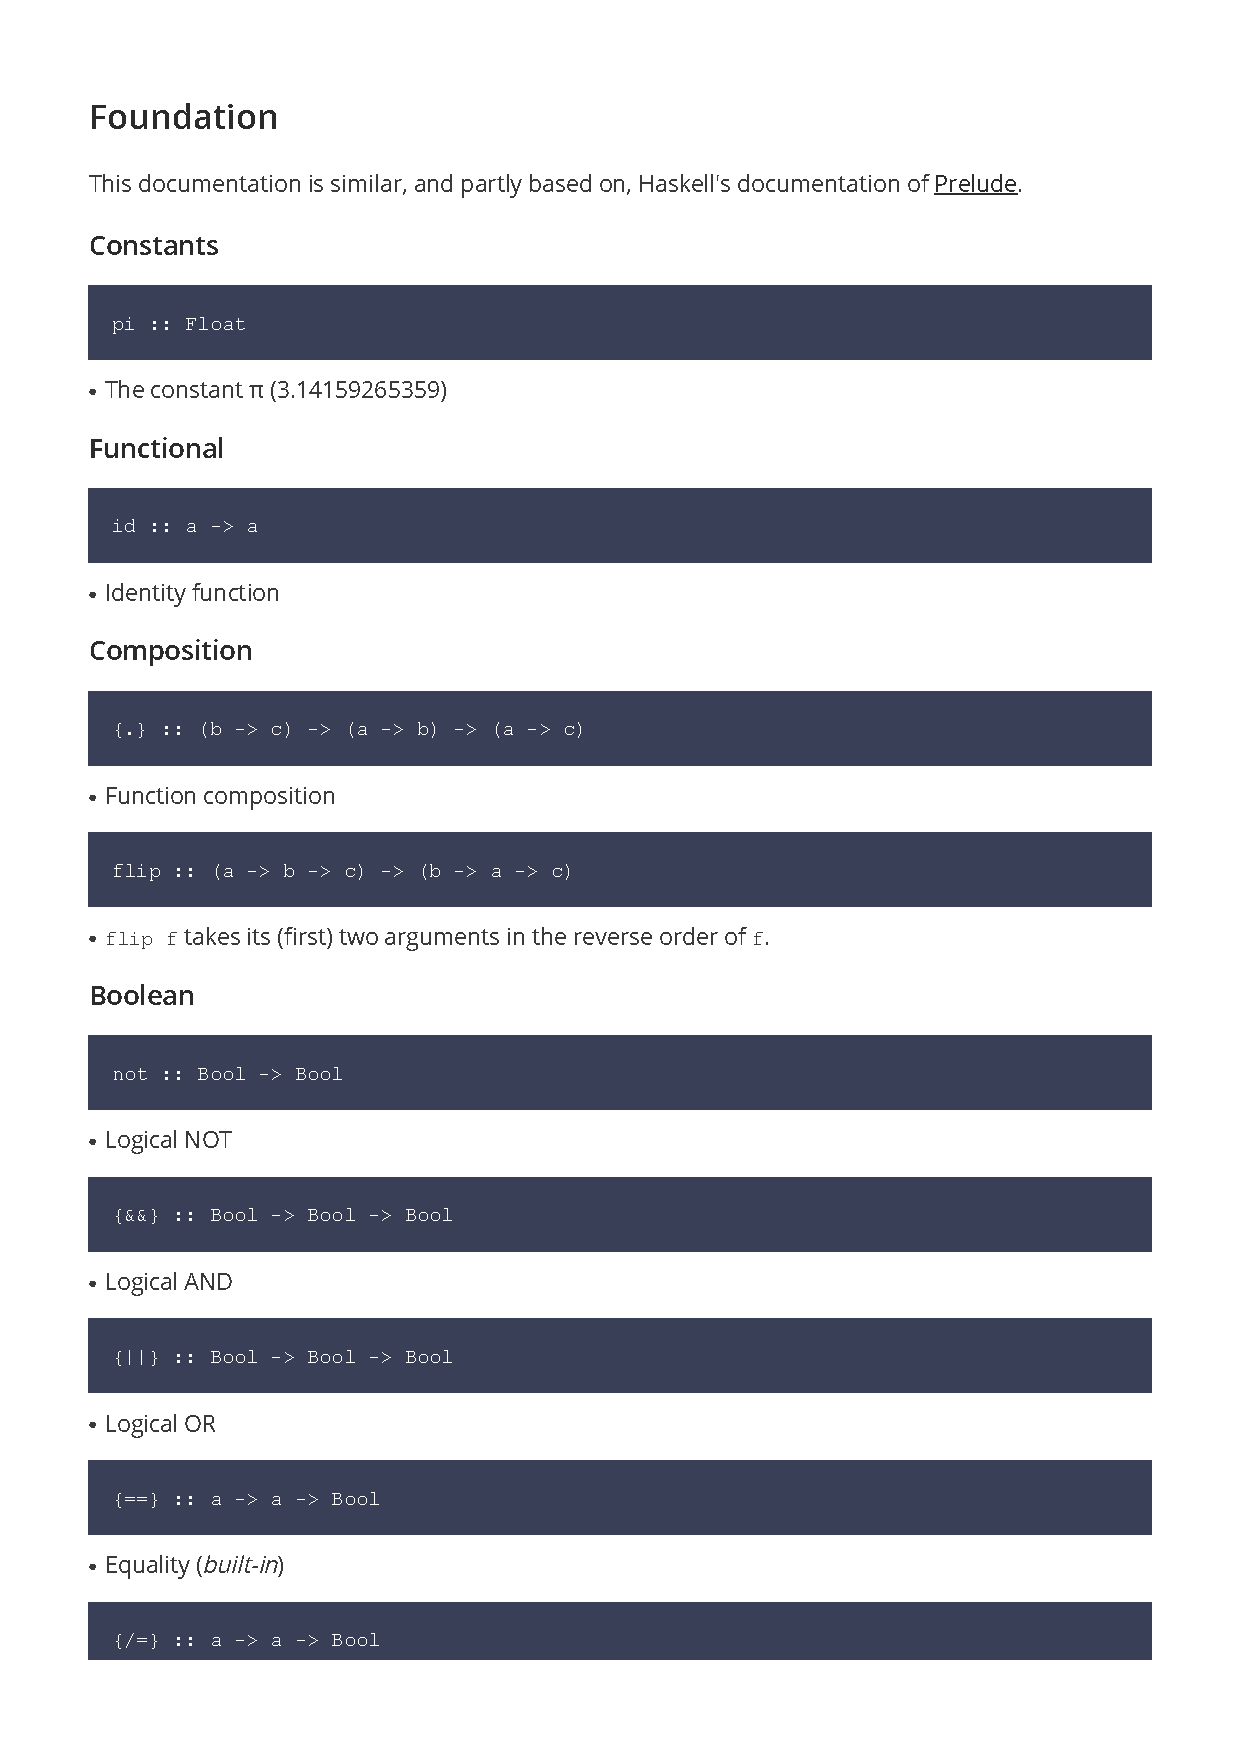
\includepdf[pages=-]{appendices/foundation-doc.pdf}



\end{document}
